\section{Búsqueda de contrastes}

% Definir que es un contraste, que tiene un uso significativo en una region más que en otra. LAs alternativas que propusimos, z test binomial.
Una palabra tiene un contraste cuando esta tiene un uso con diferencias significativas en
distintas regiones. En este trabajo nos propusimos crear un listado con palabras con contrastes que tengan
importancia a nivel lingüístico. En este sentido, los nombres de personas, lugares u organizaciones no 
fueron considerados de interés a pesar de tener contrastes en su uso.
Este listado fue ordenado por una métrica que capte en un único valor el nivel contrastivo. De esta manera, 
se seleccionó un subconjunto de palabras, de acuerdo a la métrica, el cual fue analizado manualmente en otros textos por la Academia Argentina de Letras.

El primer acercamiento para ver el contraste de las palabras lo realizamos comparando las frecuencias de las palabras 
en cada par de provincias de la Argentina. Para esto calculamos, por cada palabra, la frecuencia de ocurrencias sobre cada una de las dos provincias. La mayor frecuencia de ambas, la llamamos frecuencia máxima y a la menor, la frecuencia mínima. Luego el cociente entre la frecuencia máxima y la frecuencia mínima tiene como resultado lo que llamamos \textit{maxDif}. En caso de que en una de las dos provincias no se haya 
recolectado tuits con esa palabra, se tomaba como frecuencia mínima a la frecuencia mínima distinta de 0 de todas las palabras generadas en esa provincia. Así se evitó la división por cero. Esta métrica se resumen en la ecuación \ref{eq:maxDif}.


\begin{equation}
  \label{eq:maxDif} 
  maxDif(w,p_1,p_2) = \frac{F_{max}(w,p_1,p_2)}{F_{Min}(w,p_1,p_2)}
\end{equation}
donde 
\begin{equation}
F_{max}(w) = \max(frec(w,p_1),frec(w,p_2))
\end{equation}

%TODO: arreglar el overfull OK
\begin{equation}
 F_{min}(w) = \left\{ \begin{array}{ll}
             \min(frec(w,p_1),frec(w,p_2))  \text{ si } frec(w,p_1) * frec(w,p_2) > 0  & \\
             \\
             \min(frec(w,p))  \forall w \in palabras(p) , \text{ con } p=\{p_1,p_2\} \setminus \{P_{max}\} \text{sino} &  \\
             \end{array}
   \right.
\end{equation}
   donde $P_{max}$ es la provincia que tiene la mayor frecuencia de ambas.



De esa manera se ordenó el listado de cada par de provincias teniendo en cuenta la división de frecuencias. 
Sin embargo, este método imposibilitaba el trabajo manual para la Academia Argentina de Letras que debía mirar estos listados y hacer un análisis más exhaustivo sobre las palabras con mayor diferencia de frecuencias, debido a que había $\binom{23}{2} = 253$
listados (o equivalentemente 253 columnas en un mismo listado) a analizar. Además la métrica solo permitía saber si había un contraste entre dos provincias, pero no se podía tener en cuenta la frecuencia de la palabra en el resto de las provincias. 
% Mencionar que la idea era realizar un z test para obtener las palabras más significativas.
En consecuencia las palabras se encontraban repetidas en los distintos listados y con diferentes valores de \textit{maxDif}, lo cual hacía muy difícil poder identificar en que regiones había una diferencia significativa de frecuencias.
Debido a esto decidimos realizar un nuevo enfoque para encontrar las palabras con alta contrastividad en las distintas regiones, de manera que una métrica pueda reflejar el nivel de contrastividad de la palabra en un único valor. En primer lugar intentamos modificar la métrica \textit{maxDif} de la siguiente manera: 
Sea $f_{max}(w)$ la frecuencia máxima entre las frecuencias de todas las provincias y sea $f_{min}$ la frecuencia mínima distinta de $0$ sobre todas las provincias, luego la métrica generalizada \textit{$maxDif_g$} se puede definir como

\begin{equation}
 maxDif_g(w) = \frac{f_{max}(w)}{f_{min}(w)}
 \label{eq:maxDifg}  
\end{equation} 

Si bien esta métrica logra resumir en un único valor la diferencia de frecuencias, sigue sin considerar la dispersión de las frecuencias en todas las provincias.
Por este motivo, nos enfocamos en analizar el contraste de frecuencias de palabras sobre las provincias a través de una métrica superadora.

\subsection{Métricas para medir el contraste en la frecuencia de las palabras}
Dado que se quieren encontrar las palabras con contrastes significativos en distintas 
regiones se propone generar una métrica basada en la cantidad de información 
para poder realizar esta tarea.

Una medida que se puede usar para comparar las frecuencias de las palabras en las diferentes regiones del país puede ser la entropía definida por Shannon ( ver en el apéndice: \ref{sub:entropiaShannon}), debido a que nos brinda un valor que informe qué tan uniforme es la distribución de las frecuencias de cada palabra. La entropía es máxima cuando la probabilidad de los eventos es equiprobable y mínima en el caso que la probabilidad de un evento es 1.
Sin embargo, la entropía como única medida tiene sus desventajas. En particular, una palabra con una sola ocurrencia en una provincia y ninguna en las demás, tiene la entropía mínima. A pesar de que nos interesan las palabras con un contraste significativo entre regiones, dentro de ellas elegiremos las que tienen mayor cantidad de ocurrencias. Es por esto que elaboramos otra métrica que tenga en cuenta la entropía, entre otras variables a tener en cuenta.


\subsection{Valor de información}
La métrica que utilizamos para ordenar los listados de palabras y detectar cuáles son
las que tienen altos contrastes en su uso en distintas regiones fue inspirada por el
trabajo de Zanette y Montemurro \cite{montemurro2010towards}.
Ellos, a diferencia de Shannon, estudiaron una relación entre una medida de la información y su función semántica en el lenguaje.
A continuación detallamos el procedimiento para calcular lo que los autores llamaron
el valor de la información:

Dado un texto dividido en $P$ partes iguales llamadas ventanas, se calcula la entropía  $H(w)$ sobre el vector de cantidad de ocurrencias en cada una de las $P$ ventanas.
Luego se define $\widehat{H(w)}$  como la entropía de una permutación aleatoria del texto y promediada por todos las posibles realizaciones de la permutación de él. 
%% TODO: CHEQUEAR LA DEFINICION DE LA ENTROPIA SHUFFLEADA

Es decir, se distribuyen uniformemente las palabras en $P$ partes y se calcula la
entropía como se hizo con el texto original. Es de esperar que en la mayoría de casos 
la entropía del texto permutado sea mayor que la medida en el calculo original. Esto 
se debe a que las palabras se distribuyen de forma más uniforme 
en las distintas partes.

Finalmente, definen al valor de la información como $I(w) = p(w) (\widehat{H(w)} - H(w))$, con $p(w)$ la frecuencia total de la palabra en el texto. 
De esta manera se les da más importancia a las palabras que son más frecuentes y a las palabras que tienen una baja entropía, ya que en estas el término de la diferencia es más grande.

Zanette et al. analizaron el valor de la información sobre tres textos, \textit{Análisis de la mente}, 
\textit{Moby Dick} y \textit{El origen de las especies} de Charles Darwin. 
En los tres libros las palabras con mayor valor de la información están 
altamente relacionadas con los temas principales.

Si bien esta métrica tiene en cuenta la frecuencia de las palabras además de la 
entropía, el texto en Twitter resulta difícil de dividir en partes iguales. 
Esto es porque la división está pensada para dividir el texto en secciones que 
posiblemente hablen de distintos temas y nuestros textos son tuits que por lo general no superan las 10 palabras.
Otra dificultad que surge de esta métrica es la imposibilidad de realizar la media 
de todas las posibles permutaciones del texto por la limitación computacional ya que 
tenemos una cantidad muy grande de datos. Es por eso que diseñamos una métrica similar basada en una aproximación de la entropía máxima de una palabra.

Podemos pensar a las palabras del texto como una variable aleatoria $W$, donde cada palabra $w$ tiene una probabilidad de aparición en una provincia dada de la Argentina. Esta probabilidad la aproximamos con la frecuencia en la que aparece, es decir la cantidad de ocurrencias de la palabra dividida por la cantidad de palabras totales.
Por otro lado sea $P$ una variable aleatoria que cuenta la cantidad de personas que 
utilizan la palabra $p$ en cada provincia.

\medskip

Luego, sea $cant_w(p)$ igual al logaritmo sobre la cantidad de ocurrencias de esa palabra en toda la Argentina, es decir $cant_w(p) = \log_2(cantidadOcurrencias(p))$ .y sean las constantes $MIN_w$ y $MAX_w$ definidas de la siguiente manera:


% \noindent\begin{minipage}{.5\linewidth}
% \begin{equation}
% MIN_W = \min\limits_{p \in Palabras} cant_w(w)
% \end{equation}
% \end{minipage}%
% \begin{minipage}{.5\linewidth}
% \begin{equation}
%   MAX_W = \max\limits_{p \in Palabras} cant_w(w)
% \end{equation}
% \end{minipage}

\begin{equation}
MIN_W = \min\limits_{p \in Palabras} cant_w(w)
\end{equation}

\begin{equation}
  MAX_W = \max\limits_{p \in Palabras} cant_w(w)
\end{equation}

Realizamos una normalización lineal de la función $cant_w$, 

\begin{equation}
norm_{w}(p) = \frac{cant_w(p)- MIN_W }{MAX_W - MIN_W}
\label{eq:norm1}
\end{equation}

De esta manera, $norm_w$ tiene su imagen en el rango $[0,1]$, tomando el valor $0$ sobre la palabra que tiene la cantidad de ocurrencias máxima y toma el valor $1$ cuando se aplica a la palabra con menor cantidad de ocurrencias. Vale la pena aclarar, que tomamos $40$ como umbral mínimo de cantidad de ocurrencias de las palabras para ser estudiadas.
A partir de la función $norm_w$ definimos el valor de la información de las palabras $I_w$ como:

\begin{equation}
I_w(w) = norm_{w}(w) * (\widehat{H}_{w}(w) - H_{w}(w)) \\
\label{eq:iw}
\end{equation}

siendo $H_w(w)$ la función de entropía calculada sobre las cantidades de ocurrencias de la palabra $w$ sobre las 23 provincias argentinas. De forma similar $\widehat{H}$ es la función de entropía sobre las cantidades de ocurrencias simuladas en todas las provincias a partir de una distribución multinomial. Elegimos esta distribución ya que con esta se distribuye la suma de los valores de la variable aleatoria, en nuestro caso la cantidad de ocurrencias de la palabra $w$, de forma uniforme.%TODO: explicar más en detalle

Ahora bien, una determinada provincia o región pueden tener muchas ocurrencias de una palabra formuladas por algunos pocos usuarios que utilizan constantemente el término. Un ejemplo de esto podrían ser bots que escriben automáticamente textos iguales (o similares) en grandes cantidades. Otra posible causa de este fenómeno podría ser la de usuarios que hablan de personas, lugares o marcas de forma constante.
Es por esto que realizamos una métrica similar que tenga en cuenta la diferencia de la entropía sobre la cantidad de personas que utilizan la palabra . Agregandole el término $norm_u$, que es la constante normalizadora de la cantidad de usuarios descripta en la ecuación \ref{eq:norm2} obtenemos el valor de la información de las personas $I_u$,

\begin{equation}
I_u(w) = norm_{u}(w) * (\widehat{H}_{u}(u) - H_{u}(w))
\label{eq:iu}
\end{equation}

Donde,
\begin{equation}
norm_{u}(w) = \frac{cant_u(w)- MIN_U }{MAX_U - MIN_U}
\label{eq:norm2}
\end{equation}
\begin{equation}
 MIN_U = \min\limits_{p \in Palabras} cant_u(p)
\end{equation}
\begin{equation}
  MAX_U = \max\limits_{p \in Palabras} cant_u(p)
\end{equation}

y $cant_u(p)$ es el logaritmo sobre  la cantidad de usuarios que utilizan dicha palabra en la Argentina, es decir $cant_u(p)= \log_2(cantidadUsuarios(p)))$.

Debido a que queremos tener en cuenta tanto a la variación de la cantidad de ocurrencias de la palabra como a la variación de la cantidad de usuarios, elegimos como métrica la multiplicación de ambas métricas definidas, es decir  

\begin{equation}
%I(w) =  norm_{p}(w) * norm_{u}(w) * (\widehat{H}_{w}(w) - H_{w}(w)) * (\widehat{H}_{p}(w) - H_{p}(w)) \\
I(w) =  I_w(w) * I_u(w)\\
\label{eq:ivalor}
\end{equation}

Es importante aclarar que tanto $norm_{w}$ como $norm_{u}$ realizan una normalización del logaritmo de esas variables. Esto se debe a que el logaritmo genera una dispersión tal que agrupa los valores altos que se encontraban muy dispersos mientras que separa los valores pequeños que estaban concentrados. Esto se puede ver en las figuras \ref{fig:cantNormUsuarios} y \ref{fig:cantNormPalabras}.


%TODO: ejemplificar la variacion de la entropia.  La variacion de la entropia se puede ver como una cantidad que mide cuanta información se necesita para poder obtener esa distribución
% Si las cantidades de ocurrencias (o de personas que utilizan) de un término están distribuidas uniformemente a través de todas las provincias, quiere decir que no aporta demasiada información 

\begin{figure}[!ht]\centering
  \begin{subfigure}[t]{0.49\textwidth}
    \includegraphics[width=\linewidth]{./images/DistribucionOcurrenciasPalabrasAnotaciones.pdf}
    \caption{}
    \label{fig:cantPalabras} 
   \end{subfigure}
   \begin{subfigure}[t]{0.49\textwidth}
    \includegraphics[width=\linewidth]{images2/cantUsuarios_sinFiltro.pdf}
    \caption{}
    \label{fig:cantPalabrasPromedio} 
   \end{subfigure}
   \caption{La figura \ref{fig:cantPalabras} muestra un histograma de la cantidad de ocurrencias de las palabras. En la figura \ref{fig:cantPalabrasPromedio} se puede observar un histograma de la cantidad de usuarios que utilizan una determinada cantidad de palabras.}  
\end{figure}

Para eliminar los valores atípicos se procedió a remover tanto las palabras que no superaran las 40 ocurrencias, como también aquellas que eran dichas por menos de 6 usuarios. La métrica se evaluó en este conjunto filtrado de palabras. 

\subsection{Frecuencia de las palabras}
\label{sub: frecuenciaPalabras}
% Ver si se hace este gráfico con todas las palabras ya que por ahora tengo el conjunto de palabras con más de 40 ocurrencias
En la figura \ref{fig:cantPalabras} graficamos la distribución de la cantidad de ocurrencias de las palabras. Podemos observar que la mayoría de las palabras ocurren poco. En particular el 50\% de las palabras ocurren menos de 139 veces. Por otro lado hay pocas palabras que ocurren mucho, por ejemplo la palabra \textit{que} o la preposición \textit{de}.


\begin{figure}[!ht]\centering
  \begin{subfigure}[t]{0.49\textwidth}
    \includegraphics[width=\linewidth]{./images2/cantNormUsuarios_sinFiltro.pdf}
    \caption{} 
    \label{fig:cantNormUsuarios} 
   \end{subfigure}
   \begin{subfigure}[t]{0.49\textwidth}
    \includegraphics[width=\linewidth]{images2/cantNormPalabras_sinFiltro.pdf}
    \caption{} 
    \label{fig:cantNormPalabras} 
   \end{subfigure}
   \caption{La figura \ref{fig:cantNormUsuarios} muestra un histograma de la normalización de la cantidad de ocurrencias de las palabras, definida como $norm_u$. La figura \ref{fig:cantNormPalabras} contiene un histograma de la normalización sobre la cantidad de usuarios que utilizan una determinada cantidad de palabras definida como $norm_w$.}
\end{figure}


\begin{table}[ht]
\centering
\label{tab:palabrasMasOcurrentes}
\begin{tabular}{ c c }
\toprule
Palabra & Cantidad de Ocurrencias \\ 
\midrule
que     & 7509160                 \\
de      & 6527014                 \\
a       & 4962492                 \\
la      & 4913854                 \\
no      & 4177810                 \\
me      & 4101998                 \\
y       & 3838370                 \\
el      & 3773455                 \\
en      & 2969783                 \\
te      & 2060662                 \\
se      & 1976027                 \\
un      & 1863075                 \\
es      & 1825892                 \\
con     & 1799979                 \\
lo      & 1712189                 \\
mi      & 1643777                 \\
por     & 1553382                 \\
los     & 1498941                 \\
para    & 1398757                 \\
las     & 1212452                 \\
\bottomrule
\end{tabular}
\caption{Cantidad de apariciones de las 20 palabras más frecuentes.}

\end{table}

Si comparamos la posición de la palabra en un listado ordenado podemos ver que  las cantidades de ocurrencias parecieran seguir una distribución zipfiana. La ley de Zipf es una ley empírica formulada por George Zipf en el año 1932 en la cual se establece una relación entre la frecuencia de una palabra con su posición dentro del listado de palabras ordenadas por frecuencia decreciente \cite{montemurro2001beyond,zipf2016human}. En particular, sea $n$ la posición de la palabra en el listado ordenado y sea $f(n)$ la cantidad de ocurrencias de la n-ésima palabra, se puede hacer la siguiente aproximación:

$$f(n) \approx \frac{A}{n^{\alpha}}$$
donde $\alpha$ toma un valor levemente mayor a 1 y $A$ es una constante normalizadora.
Entonces, bajo la ley de Zipf uno puede saber que la frecuencia de la segunda palabra más dicha en un corpus, es aproximadamente la mitad que la primera. La palabra con posición 3 en el listado ordenado por frecuencias, va a tener aproximadamente la tercera parte de la cantidad de ocurrencias que la primera y así sucesivamente. De esta manera hay una relación lineal entre el logaritmo de la posición del listado ordenado por frecuencias y el logaritmo de la cantidad de ocurrencias de cada palabra.
% TODO: escribirlo en ecuación,
Otra forma de utilizar esta ley empírica es la siguiente:
sabiendo la posición de una palabra \textit{w} en el listado ordenado por frecuencias de un corpus \textbf{A} y sabiendo la cantidad de palabras totales de un corpus \textbf{B}, puede estimarse la cantidad de ocurrencias de \textit{w} en el corpus \textbf{B}.
%TODO: HACER EJEMPLO de calculo de frecuencias a traves de la frecuencia de nuestro corpus
%TODO: chequar ecuación de ley de zipf

\begin{figure}[!ht]
\centering
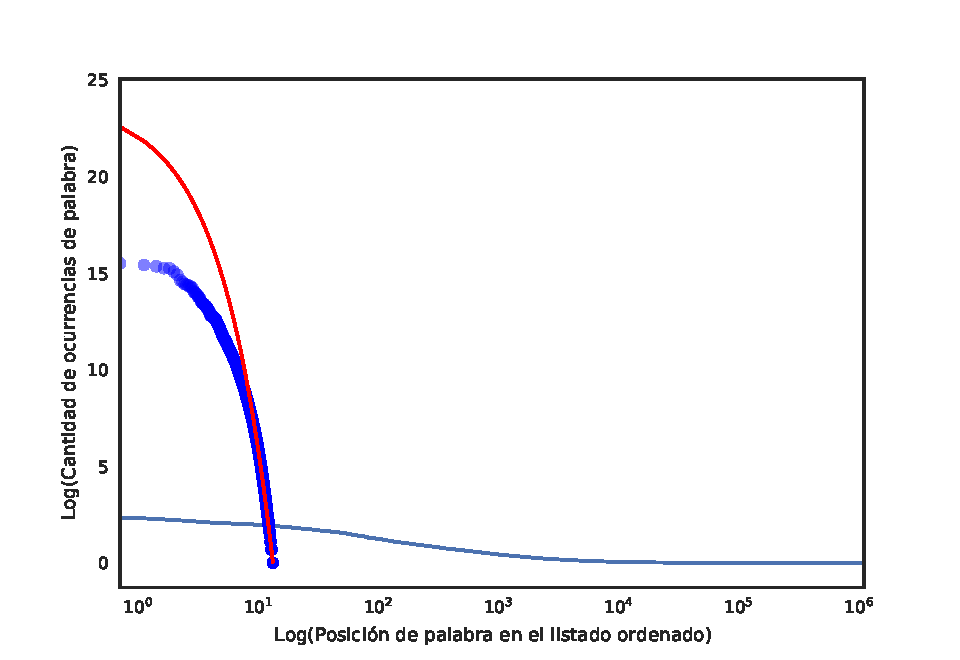
\includegraphics[width=0.5\textwidth]{images2/zipf_sinFiltro.pdf}
\caption{Cantidad de Ocurrencias de palabra vs posición en listado ordenado. Se aplicó el logaritmo natural a las cantidades de ocurrencias, como también a los valores de las posiciones para mostrar la proporcionalidad entre $f(n)$ y $\frac{1}{n^{\alpha}}$.} 
\label{fig:zipf} 
\end{figure}



%Qué resultados obtuvimos del análisis en cuestión. Acá vamos a poner qué palabras fueron significativas, dónde lo fueron, y demás.

% Distribucion de entropía vs frecuencia  
% Distribucion de frecuencias de las palabras
% Distr entropia
% de valor de la inf. a partir de los 5000 se ve que se estanca (graficar hasta 10**5)

% subsection de la region de las palabras --> muestro tabla
% se muestra que las regiones son contiguas geograficamente (hablarlo con santiago)

% Las palabras que se vieron, las primeras generalmente se refieren a lugares o gentilicios



% ver los graficos que hace zanette en su paper

% se busco el dataset de localidades para filtrar las palabras que son lugares

\section{Distribución de la entropía}
Teniendo el listado de palabras hicimos un cálculo de entropía tomando en cada provincia la cantidad de ocurrencias de cada palabra. En la figura \ref{fig:entropiaPalabras} podemos observar la distribución del valor de la entropía sobre todas las cantidades de ocurrencias de las palabras con más de 40 apariciones y dichas por más de 5 usuarios. 

Podemos ver que la mayor parte de las palabras tienen un valor de entropía entre 2.5 y 3. Esto quiere decir que hay un gran conjunto de palabras que tiene una cantidad de ocurrencias relativamente uniforme a lo largo de todas las provincias. Sin embargo, hay otro conjunto de palabras que tienen una entropía menor a 2, la cual podemos considerar como baja. Estas últimas palabras serán las que tienen mayor interés debido a que tienen una variación marcada en cuanto a su utilización en las distintas regiones. El máximo valor alcanzado de la entropía es de $3.1350$ con la palabra \textit{el}. Como aclaración la entropía calculada se realizó con logaritmos naturales, por lo tanto el máximo valor posible es de  $ln(23) = 3.1355$ donde habría una distribución uniforme en la cantidad de ocurrencias sobre las 23 provincias argentinas.

Tener en cuenta únicamente a la entropía de las palabras nos puede generar la detección de palabras que no son de interés, ya sea porque no ocurren una cantidad significativa de veces o porque la variación de las ocurrencias en las distintas provincias se debe solamente a pocos usuarios que la utilizan mucho. Es por esto que también se calculó la entropía teniendo como variable la cantidad de personas que utilizaron cierto término en una determinada provincia.


\begin{figure}[ht]
\centering
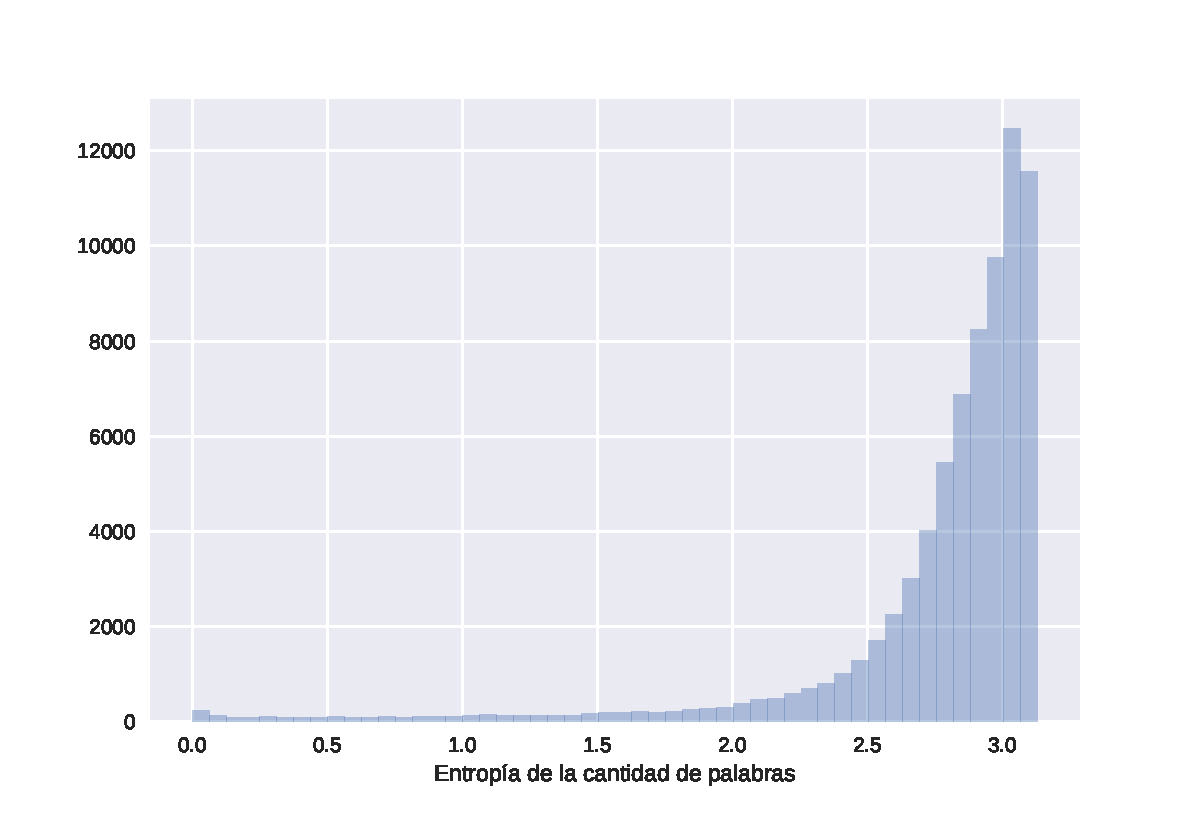
\includegraphics[width=1.0\textwidth]{./images/DistribucionEntropia.pdf}
\caption{Histograma del valor de la entropía de las palabras ($H_w$).} 
\label{fig:entropiaPalabras} 
\end{figure}



\section{Distribución del valor de la información}
\label{sec:ValorDeLaInformacion}
En el gráfico \ref{fig:infoValue} se muestra una clara relación entre la cantidad de ocurrencias que tiene una palabra y su valor de la información, indicado por el color: cuanto más oscuro más alto el valor. A su vez, se nota que el valor de la información suele ser mayor a medida que el valor de la entropía es menor. Esto no siempre es el caso debido a que hay palabras que tiene una entropía de palabras baja, pero sin embargo la entropía de personas es alta logrando que el valor de la información sea bajo.

\begin{figure}[ht]
\centering
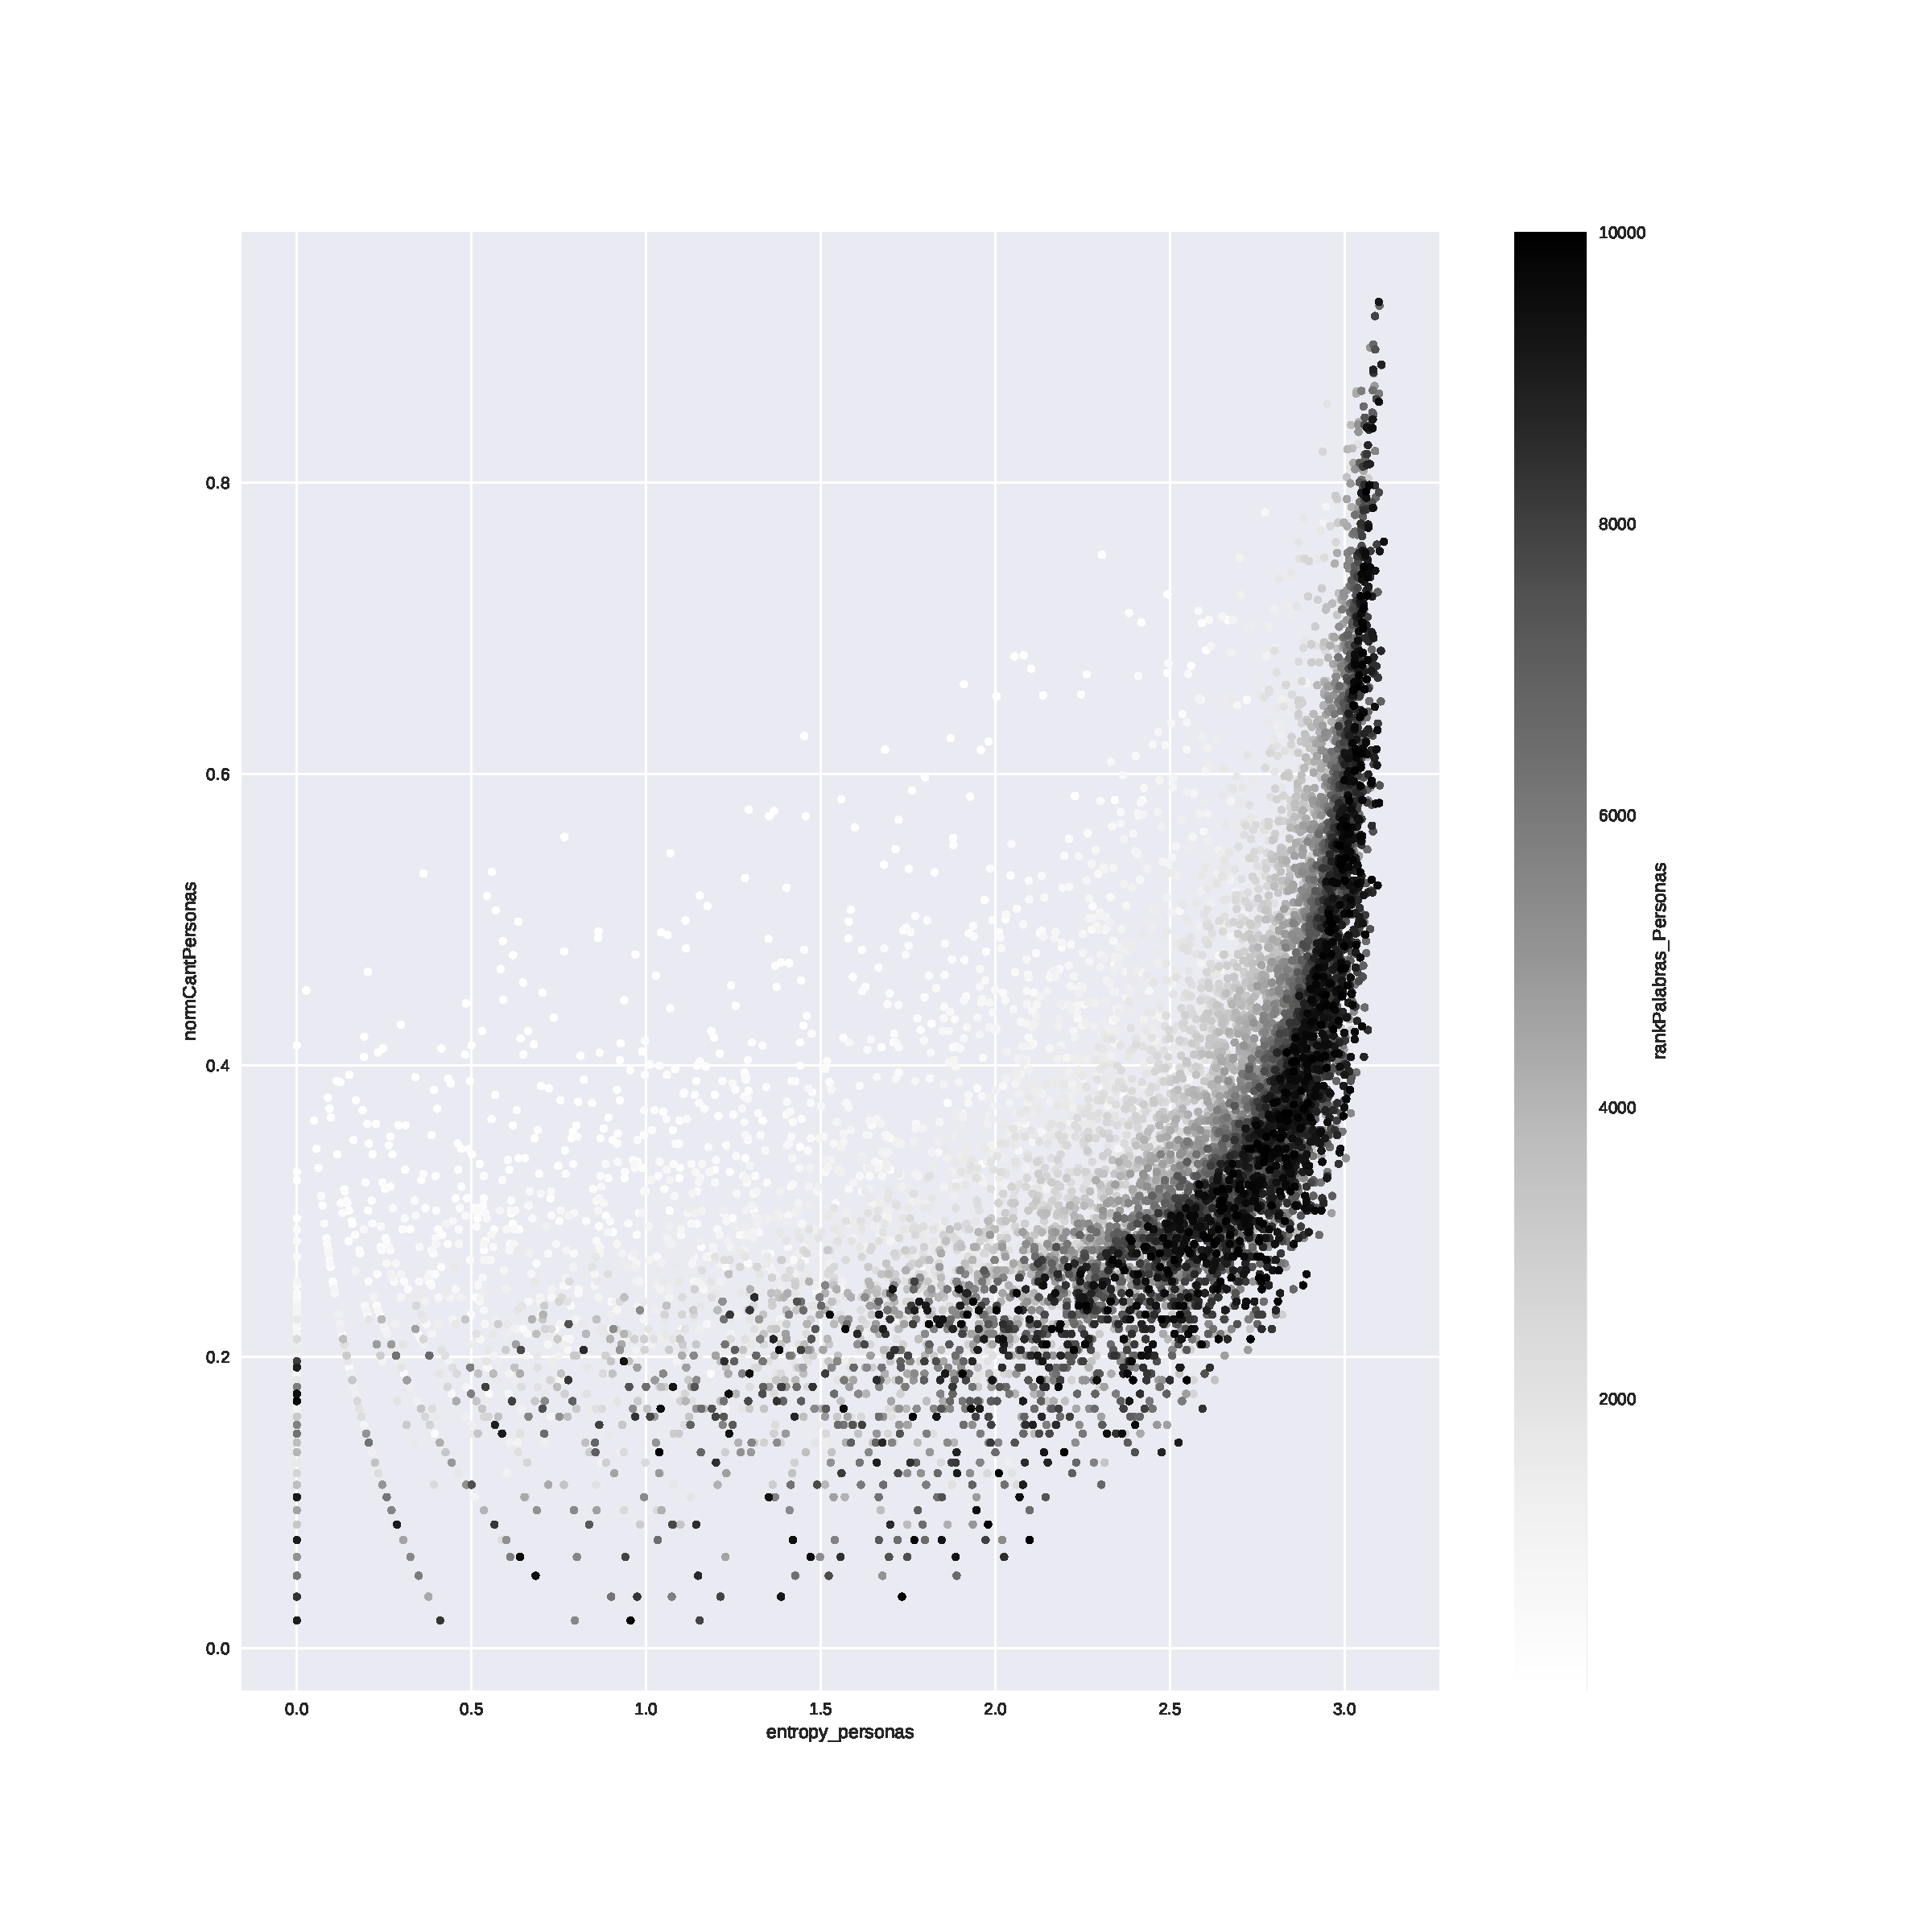
\includegraphics[width=1.0\textwidth]{./images/entropiaPersonasxNormCantPersonas.pdf}
\caption{Gráfico de dispersión que muestra la posición en el listado ordenado según el valor de la información a partir de la escala cromática. Las posiciones más bajas aparecen más blancas. A su vez se muestra para cada palabra el valor de la entropía de las personas ($H_u$) y la cantidad normalizada de personas que utiliza dicho término($norm_p$). } 
\label{fig:infoValue} 
\end{figure}

En la figura \ref{fig:ivalue} se puede ver el valor de la información según la posición en la que se encuentra en el listado ordenado por la métrica. Notamos que el valor se estabiliza aproximadamente a partir de la palabra cuya posición es 4000 acercándose a 0.


\begin{figure}
\centering
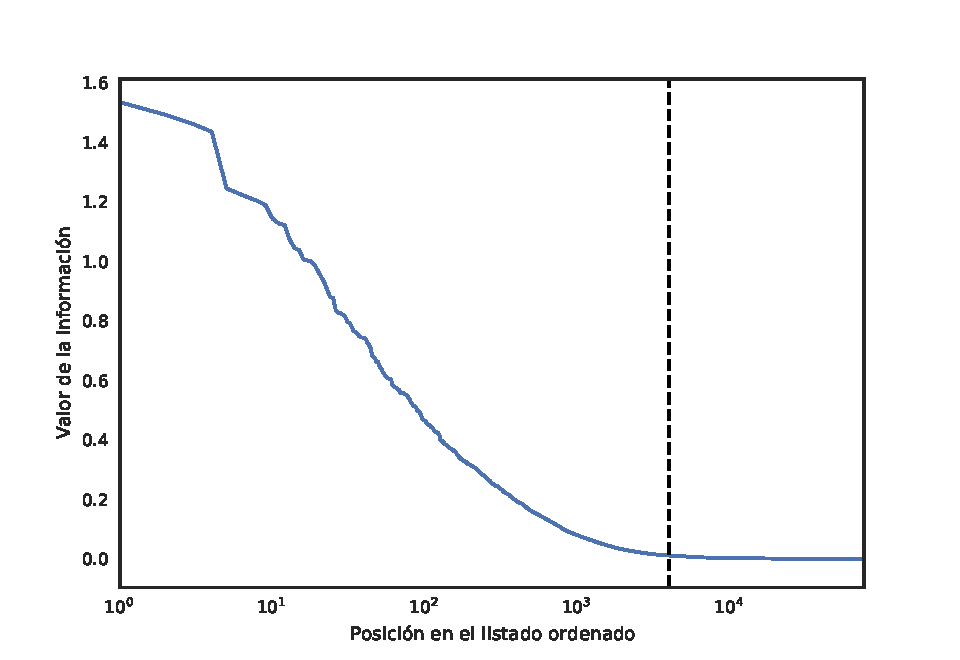
\includegraphics[width=0.9\textwidth]{./images/train/conFiltro/valorInformacionCorte.pdf}
\caption{Distribución del valor de la información según la posición de la palabra en el listado de palabras. El gráfico se realizó sobre el conjunto de palabras cuya cantidad de ocurrencias era mayor a 40 y la cantidad de usuarios que utilizaron cada término era mayor a 5. } 
\label{fig:ivalue}
\end{figure}


\section{Proporción acumulada de ocurrencias} % (fold)
\label{proporcionDeOcurrencias}
Además de la detección de las palabras contrastivas en su uso, nos interesa saber en que regiones se utilizan más. Para esto ordenamos, por cada palabra, las provincias de acuerdo a la cantidad de menciones, formando una lista de provincias: $ps = p_1,p_2,...,p_{23}$. Luego elegimos al conjunto de provincias que superen un cierto porcentaje de todas las ocurrencias. Para identificar cuál debiera ser ese porcentaje hicimos lo siguiente:

Por cada palabra, calculamos el porcentaje de ocurrencias sobre los conjuntos de $n$ provincias, variando $n$ de $1$ a $23$, a partir de las provincias ordenadas $ps$. Es decir, por cada región formada por una determinada cantidad de provincias calculamos el mayor porcentaje posible de ocurrencias de una palabra dada.
En la figura \ref{fig:propAcum} mostramos la proporción acumulada de las palabras, tomando diferentes muestras de palabras. Es notable la diferencia de proporciones acumuladas según la muestra de palabras. Solamente con una provincia para cada palabra ya se puede cubrir, en promedio, el 76\% del total de ocurrencias sobre las mil palabras con mayor valor de nuestra métrica.

En el gráfico \ref{fig:propAcum5000} se observa que la variación del cubrimiento de ocurrencias es menor a medida que se aumenta la cantidad de provincias. 


\begin{figure}\centering
    \includegraphics[width=0.9\textwidth]{images/PropAcumSinCandidatas.pdf}
    \caption{Proporción de ocurrencias acumulada según la muestra de palabras. El número de la leyenda indica la cantidad de palabras contrastivas elegidas para la muestra respectiva, siempre seleccionando las más contrastivas según la métrica.} 
    \label{fig:propAcum} 
\end{figure}


\begin{figure}[ht]\centering
    \includegraphics[width=0.95\textwidth]{images/PropAcum5000SinCandidatas.pdf}
    \caption{Variación de la proporción de ocurrencias acumulada a partir de la muestra con las primeras 5000 palabras con mayor valor de la información.} 
    \label{fig:propAcum5000} 
\end{figure}

